\section{双层优化}
\label{sec:opt-mmb-bilevel}

极小极大问题中，内层对手只关心与外层相反的同一个目标。还有一类问题，内层有它自己的目标：选择正则强度时，内层用训练损失拟合参数，外层再用验证损失评价拟合结果。外层变量要先经过一次完整的优化才能被评价，外层目标是“内层解”的函数。本节先说明这个函数在什么条件下才有定义，再给出两种计算其导数的方法，最后讨论外层求解和结果核验。

\subsection{内层选解与外层目标}
\label{sec:opt-mmb-bilevel-selection}

\paragraph{一个正则参数例}
设只有一个训练观测$3$和一个验证观测$1$，用标量参数$x$拟合，训练时加岭正则$\frac\theta2x^2$，$\theta\geq0$：
\begin{equation}
\label{eq:opt-mmb-ridge-bilevel}
L_{\mathrm{in}}(x,\theta)=\tfrac12(x-3)^2+\tfrac\theta2x^2,\qquad
L_{\mathrm{out}}(x)=\tfrac12(x-1)^2.
\end{equation}
内层对每个$\theta$有唯一最小点$x^\star(\theta)=3/(1+\theta)$，外层要最小化$J(\theta)=L_{\mathrm{out}}(x^\star(\theta))=\frac12\bigl(\frac3{1+\theta}-1\bigr)^2$，最小点是$\theta=2$，此时$x^\star=1$恰好拟合验证观测。这里$x$是内层变量，由训练决定；$\theta$是外层变量，由验证决定。外层从不直接改变$x$，只能通过改变内层问题间接影响它。

\paragraph{内层多解时的选解规则}
一般地，记外层变量$\bm\theta\in\Theta\subseteq\mathbb R^p$，内层变量$\bm x\in\mathbb R^d$，内层解集
\[
S(\bm\theta)=\argmin_{\bm x\in\mathbb R^d}L_{\mathrm{in}}(\bm x,\bm\theta).
\]
若$S(\bm\theta)$总是单点$\{\bm x^\star(\bm\theta)\}$，外层目标$J(\bm\theta)=L_{\mathrm{out}}(\bm x^\star(\bm\theta),\bm\theta)$有明确定义。$S(\bm\theta)$含多个点时，“内层解代入外层”还不是一个函数，必须补充选解规则。常见的三种是：乐观规则取$J_{\mathrm{opt}}(\bm\theta)=\inf_{\bm x\in S(\bm\theta)}L_{\mathrm{out}}(\bm x,\bm\theta)$，假定内层会配合外层；悲观规则取$J_{\mathrm{pes}}(\bm\theta)=\sup_{\bm x\in S(\bm\theta)}L_{\mathrm{out}}(\bm x,\bm\theta)$，按最不利的内层解评价；算法规则取某个指定算法从指定初值出发得到的解。

\begin{definition}[双层优化问题]
\label{def:opt-mmb-bilevel}
给定外层可行域$\Theta$、内层目标$L_{\mathrm{in}}$、外层评价$L_{\mathrm{out}}$以及一个选解规则，由选解规则确定的外层目标记为$J(\bm\theta)$，问题$\min_{\bm\theta\in\Theta}J(\bm\theta)$称为\term{双层优化}（bilevel optimization）问题。内层解唯一时，选解规则可以省略。
\end{definition}

图~\ref{fig:opt-mmb-inner-selection}给出一个规则确实起作用的例子。取二维内层变量与外层目标点$\bm c=(1.5,0.5)$：
\[
L_{\mathrm{in}}(\bm x,\theta)=\tfrac12(x_1+x_2-2)^2+\tfrac\theta2\lVert\bm x\rVert_2^2,\qquad
L_{\mathrm{out}}(\bm x)=\tfrac12\lVert\bm x-\bm c\rVert_2^2.
\]
$\theta>0$时内层强凸，令梯度$(x_1+x_2-2)(1,1)+\theta\bm x$为零，得唯一解$\frac2{2+\theta}(1,1)$。$\theta=0$时内层解集是整条直线$x_1+x_2=2$，三种规则给出不同答案：乐观规则选$\bm c$本身，外层值为$0$；悲观规则面对的直线无界，外层值为$+\infty$；从原点出发的梯度下降，每步的梯度都平行于$(1,1)$，迭代停在最小范数解$(1,1)$，外层值为$\frac14$。当$\theta\to0^+$时唯一解趋于$(1,1)$，外层值趋于$\frac14$，所以只有算法规则与正则化路径衔接，乐观规则下的$J$在$\theta=0$处不连续。

\begin{figure}[!htbp]
  \centering
  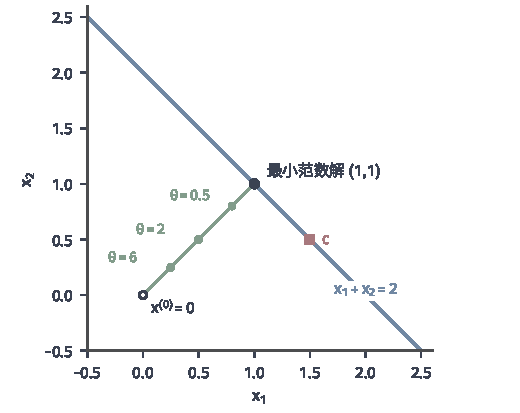
\includegraphics[width=88mm]{figures/03-optimization-evolution-and-signals/01-optimization/matplotlib/c7-inner-selection/figure.pdf}
  \caption{内层多解时的选解。蓝线是$\theta=0$时内层$\frac12(x_1+x_2-2)^2$的解集；绿线是$\theta>0$时的唯一解$\frac2{2+\theta}(1,1)$随$\theta$的轨迹，标出$\theta=0.5,2,6$三点。$\theta\to0^+$时它趋于最小范数解$(1,1)$，从原点出发的梯度下降也停在这里；外层目标点$\bm c=(1.5,0.5)$虽在解集上，只有乐观规则会选它。}
  \label{fig:opt-mmb-inner-selection}
\end{figure}

\paragraph{三种外层目标}
即使内层损失相同，实际计算中也会出现三个不同的外层目标。第一是理想的全局选解目标$J$，它要求内层被精确地全局求解。第二是局部分支目标$\widehat J$：内层非凸时，我们往往只能沿某个局部极小点随$\bm\theta$连续变化的分支计算，这一分支未必处处是全局最优解。第三是有限步目标$J_T(\bm\theta)=L_{\mathrm{out}}(\bm x^{(T)}(\bm\theta),\bm\theta)$，其中$\bm x^{(T)}(\bm\theta)$是内层算法从给定初值运行$T$步的输出。三者的最小点可以不同，导数也可以不同。上面的二维例子还说明，内层最优值相同不等于外层评价相同：直线$x_1+x_2=2$上每一点的内层损失都是零，外层值却从$0$到$+\infty$都有。外层目标对$\bm\theta$的梯度称为\term{超梯度}（hypergradient），下面两小节分别对$J_T$和$\widehat J$求超梯度，图~\ref{fig:opt-mmb-bilevel-chain}把两条计算路线并排画出。

\begin{figure*}[!htbp]
  \centering
  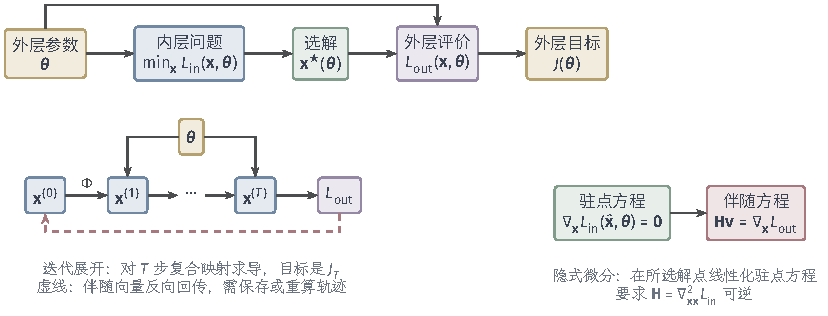
\includegraphics[width=140.1mm]{figures/03-optimization-evolution-and-signals/01-optimization/tikz/c7-bilevel-chain/figure.pdf}
  \caption{双层问题的复合结构与两种超梯度。上行：外层参数$\bm\theta$同时进入内层问题和外层评价，内层按选解规则给出$\bm x^\star(\bm\theta)$，外层目标$J$是两者的复合。左下：迭代展开把$T$步内层更新$\Phi$看成依赖$\bm\theta$的复合映射，虚线表示反向累计时伴随向量从外层评价逐步传回初值，需要保存或重算整条轨迹。右下：隐式微分只在所选解点处线性化驻点方程，解一个以内层Hessian为系数的伴随方程。}
  \label{fig:opt-mmb-bilevel-chain}
\end{figure*}

\subsection{迭代展开法}
\label{sec:opt-mmb-unrolling}

\paragraph{把有限步算法看成复合映射}
设内层用固定步长$\eta$的梯度下降，$L_{\mathrm{in}}$二阶连续可微：
\[
\bm x^{(t+1)}=\Phi(\bm x^{(t)},\bm\theta)=\bm x^{(t)}-\eta\nabla_{\bm x}L_{\mathrm{in}}(\bm x^{(t)},\bm\theta),\qquad t=0,\dots,T-1.
\]
$\bm x^{(T)}$是$\bm\theta$经过$T$层复合得到的函数，对它求导只需反复使用链式法则，这就是\term{迭代展开法}（unrolled differentiation）。记$\bm D^{(t)}=\partial\bm x^{(t)}/\partial\bm\theta\in\mathbb R^{d\times p}$，
\[
\bm A^{(t)}=\bm I-\eta\nabla^2_{\bm x\bm x}L_{\mathrm{in}}(\bm x^{(t)},\bm\theta),\qquad
\bm C^{(t)}=-\eta\nabla^2_{\bm x\bm\theta}L_{\mathrm{in}}(\bm x^{(t)},\bm\theta)\in\mathbb R^{d\times p}.
\]
对更新式两边关于$\bm\theta$求导，$\bm x^{(t)}$本身依赖$\bm\theta$，所以
\begin{equation}
\label{eq:opt-mmb-forward-sensitivity}
\begin{aligned}
\bm D^{(t+1)}&=\bm A^{(t)}\bm D^{(t)}+\bm C^{(t)},\\
\nabla J_T(\bm\theta)&=(\bm D^{(T)})^\top\nabla_{\bm x}L_{\mathrm{out}}(\bm x^{(T)},\bm\theta)+\nabla_{\bm\theta}L_{\mathrm{out}}(\bm x^{(T)},\bm\theta).
\end{aligned}
\end{equation}
初值$\bm D^{(0)}=\partial\bm x^{(0)}/\partial\bm\theta$通常为零，但若用上一个$\bm\theta$的解热启动，初值也依赖$\bm\theta$，这一项不能丢。这里用到的多元复合函数链式法则，以及下一小节要用的隐函数定理，都可参考\BookChapterRef{chap:multivariate-calculus}{卷一“多元函数微分”章}。

\paragraph{完整状态与其他参数}
若内层用带动量或自适应统计的方法，一步更新依赖的不只是$\bm x^{(t)}$。这时要把完整状态$\bm z^{(t)}$（例如参数与动量）作为展开对象，更新写成$\bm z^{(t+1)}=\Phi_t(\bm z^{(t)},\bm\theta)$，递推改为$\bm D_{\bm z}^{(t+1)}=\partial_{\bm z}\Phi_t\,\bm D_{\bm z}^{(t)}+\partial_{\bm\theta}\Phi_t$。只对$\bm x$部分求导会漏掉动量对$\bm\theta$的依赖。若步长、动量系数本身就是外层要调的参数，它们也出现在$\partial_{\bm\theta}\Phi_t$中。更新中含有截断、符号或取最大值等运算时，复合映射只在不切换分支的区域可微，求导前要确认迭代没有落在切换点上。

\paragraph{正则参数例中的展开}
在例~\eqref{eq:opt-mmb-ridge-bilevel}中取$x^{(0)}=0$、$\eta=\frac12$。这时$\nabla^2_{xx}L_{\mathrm{in}}=1+\theta$，$\nabla^2_{x\theta}L_{\mathrm{in}}=x$，所以$A^{(t)}=1-\frac{1+\theta}2$，$C^{(t)}=-\frac12x^{(t)}$。在$\theta=0$处$A^{(t)}=\frac12$，迭代与导数依次为
\[
x^{(0)},x^{(1)},x^{(2)},x^{(3)}=0,\ \tfrac32,\ \tfrac94,\ \tfrac{21}8;\qquad
D^{(0)},D^{(1)},D^{(2)},D^{(3)}=0,\ 0,\ -\tfrac34,\ -\tfrac32.
\]
于是$J_2'(0)=(x^{(2)}-1)D^{(2)}=-\frac{15}{16}$，$J_3'(0)=-\frac{39}{16}$；而理想目标的导数是$J'(0)=(x^\star-1)\frac{\mathrm dx^\star}{\mathrm d\theta}=2\times(-3)=-6$。三个数都是正确的导数，只是对应不同的目标。$J_1$尤其特别：从$x^{(0)}=0$出发，第一步的梯度$-(3-x^{(0)})+\theta x^{(0)}=-3$与$\theta$无关，于是$x^{(1)}=\frac32$对所有$\theta$都相同，$J_1$是常数，展开一步完全看不到正则的作用。

不同的$T$还会移动外层的最小点。$x^{(2)}=\frac94-\frac34\theta$，它在$\theta=\frac53$时等于验证观测$1$，所以$J_2$的最小点是$\frac53$，而$J$的最小点是$2$。图~\ref{fig:opt-mmb-unroll}左栏画出了$x^{(T)}(\theta)$与$x^\star(\theta)$：各曲线穿过水平线$x=1$的位置就是相应外层目标的最小点，曲线在$\theta=0$处的斜率就是$D^{(T)}$。本例中$|A^{(t)}|=\frac12<1$，导数$D^{(T)}$随$T$收敛到$\mathrm dx^\star/\mathrm d\theta$；一般问题中迭代点收敛并不自动推出导数收敛，后者还需要$\bm A^{(t)}$的谱半径一致地小于$1$一类的条件。还要注意固定步长$\eta=\frac12$只在$\theta<3$时使内层迭代收敛，$\theta\geq3$时$J_T$描述的是一个发散算法的输出。

\begin{figure*}[!htbp]
  \centering
  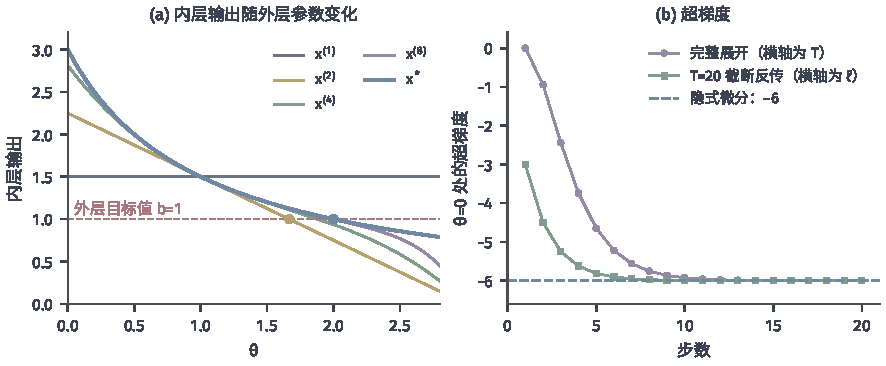
\includegraphics[width=150mm]{figures/03-optimization-evolution-and-signals/01-optimization/matplotlib/c7-unroll-vs-implicit/figure.pdf}
  \caption{正则参数例~\eqref{eq:opt-mmb-ridge-bilevel}的展开与隐式超梯度，内层梯度下降取$x^{(0)}=0$、$\eta=1/2$。(a)内层输出随$\theta$的变化：$x^{(T)}(\theta)$（$T=1,2,4,8$）与精确解$x^\star=3/(1+\theta)$；红虚线是验证观测$1$，曲线与它的交点是外层最小点，$J_2$在$\theta=5/3$、$J$在$\theta=2$；所有曲线在$\theta=1$相交，因为此时$A^{(t)}=0$，一步即得精确解。(b)$\theta=0$处的超梯度：紫线是完整展开的$J_T'(0)$随$T$的变化（$0,-15/16,-39/16,\dots$），绿线是$T=20$时只回传最后$\ell$步的截断结果，蓝虚线是隐式微分给出的$J'(0)=-6$。}
  \label{fig:opt-mmb-unroll}
\end{figure*}

\paragraph{前向灵敏度与反向累计}
递推~\eqref{eq:opt-mmb-forward-sensitivity}是前向计算：它随内层迭代同步更新$d\times p$矩阵$\bm D^{(t)}$，每步需要$\nabla^2_{\bm x\bm x}L_{\mathrm{in}}$与$p$个向量的乘积，存储$O(dp)$，不需要保存轨迹。外层参数很多时（例如每个样本一个权重），$p$与$d$同阶，这一代价不可接受。把$\nabla J_T$展开成乘积之和，可以从后往前累计：
\begin{equation}
\label{eq:opt-mmb-reverse}
\begin{aligned}
&\bm q^{(T)}=\nabla_{\bm x}L_{\mathrm{out}}(\bm x^{(T)},\bm\theta),\\
&\bm h\gets\bm h+(\bm C^{(t)})^\top\bm q^{(t+1)},\quad
\bm q^{(t)}=(\bm A^{(t)})^\top\bm q^{(t+1)},\qquad t=T-1,\dots,0,
\end{aligned}
\end{equation}
从$\bm h=\nabla_{\bm\theta}L_{\mathrm{out}}(\bm x^{(T)},\bm\theta)$开始，最后再加上初值项$(\bm D^{(0)})^\top\bm q^{(0)}$，得到的$\bm h$就是$\nabla J_T(\bm\theta)$。反向计算每步只需一次Hessian--向量积和一次混合二阶导数与向量的乘积，与$p$无关；代价是计算$\bm A^{(t)},\bm C^{(t)}$需要$\bm x^{(t)}$，必须保存整条轨迹，存储$O(Td)$。折中做法是每隔$k$步保存一个检查点，反向时从最近的检查点重算中间状态，存储约为$T/k+k$个状态，额外约一次前向计算；取$k\approx\sqrt T$时存储降到$O(\sqrt Td)$。

\paragraph{截短前向与截断反传}
为了省时，常见两种截断，它们的性质完全不同。一种是减少前向步数，用$J_{T'}$（$T'<T$）代替$J_T$：这改变了目标本身，上例中$J_2$与$J$的最小点已经相差$\frac13$。另一种是前向仍跑满$T$步，反向只回传最后$\ell$步：它近似的仍是$J_T$的导数。由$\bm D^{(T)}=\bm A^{(T-1)}\cdots\bm A^{(T-\ell)}\bm D^{(T-\ell)}+\sum_{t=T-\ell}^{T-1}\bm A^{(T-1)}\cdots\bm A^{(t+1)}\bm C^{(t)}$，被舍去的正是第一项，误差满足
\[
\lVert\text{截断误差}\rVert_2\leq\lVert\nabla_{\bm x}L_{\mathrm{out}}(\bm x^{(T)},\bm\theta)\rVert_2\,\lVert\bm A^{(T-1)}\cdots\bm A^{(T-\ell)}\rVert_2\,\lVert\bm D^{(T-\ell)}\rVert_2.
\]
内层是收缩迭代时，这一误差随$\ell$几何衰减。图~\ref{fig:opt-mmb-unroll}右栏中$A^{(t)}=\frac12$，只回传一步得到$-3$，回传约十步后已与完整展开几乎相同。

\subsection{隐式微分法}
\label{sec:opt-mmb-implicit}

迭代展开的存储和计算都随$T$增长，而且求出的是有限步目标的导数。若内层已经求解到某个非退化的局部极小点附近，可以绕过整条轨迹，直接对“梯度为零”这个方程求导。

\paragraph{选定分支上的导数}
设$\hat{\bm x}_0$是$L_{\mathrm{in}}(\cdot,\bm\theta_0)$的局部极小点，满足驻点方程$\nabla_{\bm x}L_{\mathrm{in}}(\hat{\bm x}_0,\bm\theta_0)=\bm 0$，且$L_{\mathrm{in}}$在$(\hat{\bm x}_0,\bm\theta_0)$附近二阶连续可微。把驻点方程看作关于$(\bm x,\bm\theta)$的$d$个方程，它对$\bm x$的Jacobian就是内层Hessian。

\begin{theorem}[解分支的可微性]
\label{thm:opt-mmb-implicit-branch}
若$\bm H_0=\nabla^2_{\bm x\bm x}L_{\mathrm{in}}(\hat{\bm x}_0,\bm\theta_0)$可逆，则存在$\bm\theta_0$的邻域$U$、$\hat{\bm x}_0$的邻域$V$和唯一的连续可微映射$\hat{\bm x}:U\to V$，使$\hat{\bm x}(\bm\theta_0)=\hat{\bm x}_0$且$\nabla_{\bm x}L_{\mathrm{in}}(\hat{\bm x}(\bm\theta),\bm\theta)=\bm 0$；其导数为
\begin{equation}
\label{eq:opt-mmb-implicit-derivative}
\frac{\partial\hat{\bm x}}{\partial\bm\theta}=-\bm H^{-1}\bm B,\qquad
\bm H=\nabla^2_{\bm x\bm x}L_{\mathrm{in}}(\hat{\bm x}(\bm\theta),\bm\theta),\quad
\bm B=\nabla^2_{\bm x\bm\theta}L_{\mathrm{in}}(\hat{\bm x}(\bm\theta),\bm\theta).
\end{equation}
若$\bm H_0\succ\bm 0$，则缩小$U$后，$\hat{\bm x}(\bm\theta)$都是严格局部极小点。
\end{theorem}

\begin{proof}
前半部分是卷一隐函数定理应用于方程$\nabla_{\bm x}L_{\mathrm{in}}(\bm x,\bm\theta)=\bm 0$的结论，该方程关于$\bm x$的Jacobian正是$\bm H$；对恒等式$\nabla_{\bm x}L_{\mathrm{in}}(\hat{\bm x}(\bm\theta),\bm\theta)=\bm 0$两边关于$\bm\theta$求导得$\bm H\,\partial\hat{\bm x}/\partial\bm\theta+\bm B=\bm 0$。Hessian连续而正定矩阵的最小特征值连续依赖矩阵，所以$\bm H_0\succ\bm 0$时在$\bm\theta_0$附近$\bm H\succ\bm 0$，再由第~\ref{chap:optimization}章的二阶充分条件，驻点$\hat{\bm x}(\bm\theta)$是严格局部极小点。
\end{proof}

把式~\eqref{eq:opt-mmb-implicit-derivative}代入外层链式法则，得到局部分支目标$\widehat J(\bm\theta)=L_{\mathrm{out}}(\hat{\bm x}(\bm\theta),\bm\theta)$的梯度，称为\term{隐式超梯度}（implicit hypergradient）：
\begin{equation}
\label{eq:opt-mmb-implicit-hypergradient}
\nabla\widehat J(\bm\theta)=\nabla_{\bm\theta}L_{\mathrm{out}}-\bm B^\top\bm v,\qquad
\bm H\bm v=\nabla_{\bm x}L_{\mathrm{out}},
\end{equation}
其中各导数都在$(\hat{\bm x}(\bm\theta),\bm\theta)$处取值，并用了$\bm H$的对称性。实际计算从不显式形成$\bm H^{-1}$，而是解伴随方程$\bm H\bm v=\nabla_{\bm x}L_{\mathrm{out}}$。$\bm H$正定时可用共轭梯度法，每次迭代只需一次Hessian--向量积，迭代线性求解器的做法见\BookChapterRef{chap:linear-equations-and-optimization}{卷一“线性方程与矩阵方程”章}。整个计算如算法~\ref{alg:opt-mmb-implicit}所示，它只用到解点处的信息，存储为$O(d)$，与内层跑了多少步无关。

\begin{algorithm}[隐式超梯度]
\label{alg:opt-mmb-implicit}
\begin{algorithmic}[1]
\Require 外层参数$\bm\theta$，内层求解器与容差$\varepsilon_{\mathrm{in}}$，伴随求解容差$\varepsilon_{\mathrm{lin}}$
\Ensure 近似超梯度$\tilde{\bm h}$，内层残差$\bm r_{\mathrm{in}}$与伴随残差$\bm r_{\mathrm{lin}}$
\State 求解内层到$\tilde{\bm x}$，使$\bm r_{\mathrm{in}}=\nabla_{\bm x}L_{\mathrm{in}}(\tilde{\bm x},\bm\theta)$满足$\lVert\bm r_{\mathrm{in}}\rVert_2\leq\varepsilon_{\mathrm{in}}$
\State 检查$\tilde{\bm x}$处Hessian的最小特征值（或其可靠下界）为正，否则报告分支退化
\State 用共轭梯度法近似求解$\bm H(\tilde{\bm x})\bm v=\nabla_{\bm x}L_{\mathrm{out}}(\tilde{\bm x},\bm\theta)$，得$\tilde{\bm v}$及残差$\bm r_{\mathrm{lin}}$，直到$\lVert\bm r_{\mathrm{lin}}\rVert_2\leq\varepsilon_{\mathrm{lin}}$
\State $\tilde{\bm h}\gets\nabla_{\bm\theta}L_{\mathrm{out}}(\tilde{\bm x},\bm\theta)-\bm B(\tilde{\bm x})^\top\tilde{\bm v}$
\end{algorithmic}
\end{algorithm}

在正则参数例中，$H=1+\theta$，$B=x$，伴随方程给出$v=(x-1)/(1+\theta)$，于是$\widehat J'(\theta)=-x(x-1)/(1+\theta)$。$\theta=0$、$x=3$时得$-6$，与直接对$J$求导一致，也是图~\ref{fig:opt-mmb-unroll}右栏中展开导数随$T$趋近的值。

定理~\ref{thm:opt-mmb-implicit-branch}只说明一个局部分支是可微的，并不说明这个分支就是规定的选解。内层非凸时，沿分支算出的是$\widehat J$的导数；只有当该分支在所考虑的$\bm\theta$范围内始终是全局最小点（或始终符合规定的选解规则）时，才有$\widehat J=J$。第~\ref{sec:opt-mmb-outer}小节会给出两者分离的具体例子。

\paragraph{两类残差及其放大}
算法~\ref{alg:opt-mmb-implicit}有两处近似：内层点$\tilde{\bm x}$不是精确驻点，伴随方程也只解到残差$\bm r_{\mathrm{lin}}=\bm H(\tilde{\bm x})\tilde{\bm v}-\nabla_{\bm x}L_{\mathrm{out}}(\tilde{\bm x},\bm\theta)$。为了分别追踪它们，把式~\eqref{eq:opt-mmb-implicit-hypergradient}的右端看作内层点的函数
\[
\bm h(\bm x)=\nabla_{\bm\theta}L_{\mathrm{out}}(\bm x,\bm\theta)-\bm B(\bm x)^\top\bm H(\bm x)^{-1}\nabla_{\bm x}L_{\mathrm{out}}(\bm x,\bm\theta),
\]
真值是$\bm h(\hat{\bm x})$。

\begin{lemma}[超梯度的误差分解]
\label{lem:opt-mmb-hypergradient-error}
设$N$是含$\hat{\bm x}$与$\tilde{\bm x}$的凸集，在$N$上$\nabla^2_{\bm x\bm x}L_{\mathrm{in}}(\cdot,\bm\theta)\succeq\mu\bm I$（$\mu>0$），且$\bm h$在$N$上是$K_h$-Lipschitz的。则
\[
\lVert\tilde{\bm h}-\bm h(\hat{\bm x})\rVert_2\leq\frac{K_h}{\mu}\lVert\bm r_{\mathrm{in}}\rVert_2+\frac{\lVert\bm B(\tilde{\bm x})\rVert_2}{\mu}\lVert\bm r_{\mathrm{lin}}\rVert_2.
\]
\end{lemma}

\begin{proof}
把误差拆成$\tilde{\bm h}-\bm h(\tilde{\bm x})$与$\bm h(\tilde{\bm x})-\bm h(\hat{\bm x})$。前者等于$-\bm B(\tilde{\bm x})^\top\bigl(\tilde{\bm v}-\bm H(\tilde{\bm x})^{-1}\nabla_{\bm x}L_{\mathrm{out}}\bigr)=-\bm B(\tilde{\bm x})^\top\bm H(\tilde{\bm x})^{-1}\bm r_{\mathrm{lin}}$，而$\lVert\bm H(\tilde{\bm x})^{-1}\rVert_2\leq1/\mu$。后者不超过$K_h\lVert\tilde{\bm x}-\hat{\bm x}\rVert_2$。最后，沿$N$中连接两点的线段积分Hessian得$\langle\nabla_{\bm x}L_{\mathrm{in}}(\tilde{\bm x})-\nabla_{\bm x}L_{\mathrm{in}}(\hat{\bm x}),\tilde{\bm x}-\hat{\bm x}\rangle\geq\mu\lVert\tilde{\bm x}-\hat{\bm x}\rVert_2^2$，左侧第二个梯度为零，由Cauchy--Schwarz不等式得$\lVert\tilde{\bm x}-\hat{\bm x}\rVert_2\leq\lVert\bm r_{\mathrm{in}}\rVert_2/\mu$。
\end{proof}

两项分别来自“在错误的点上求导”与“在正确的点上没解准伴随方程”，各自需要单独控制，压低其中一项并不能控制另一项。小曲率$\mu$同时放大两者，而且$K_h$本身通常也含有$1/\mu$。看一个可以直接算的例子：$L_{\mathrm{in}}(x,\theta)=\frac\mu2x^2-\theta x$，$L_{\mathrm{out}}=\frac12(x-1)^2$。这时$\hat x=\theta/\mu$，$H=\mu$，$B=-1$，$h(x)=(x-1)/\mu$。内层残差$r_{\mathrm{in}}=\mu\tilde x-\theta$造成点误差$r_{\mathrm{in}}/\mu$，再经$h$放大为$r_{\mathrm{in}}/\mu^2$；伴随残差造成$v$的误差$r_{\mathrm{lin}}/\mu$，超梯度误差也是$r_{\mathrm{lin}}/\mu$。取$\mu=0.01$、两个残差都是$10^{-4}$，前者使超梯度偏差$1$，后者偏差$0.01$。内层“几乎平坦”时，看似很小的残差也会让超梯度失去意义。

\paragraph{公式的适用边界}
式~\eqref{eq:opt-mmb-implicit-hypergradient}依赖三件事：内层无约束、解点处梯度为零、Hessian可逆。内层带约束且解在边界上时，驻点方程要换成KKT系统；活动约束集合保持不变时，可以对KKT方程组整体应用同样的隐函数论证，第~\ref{chap:constrained-optimization}章讨论了这种参数敏感性，而活动集切换的参数处解映射一般不可微。Hessian奇异时（例如两条分支在折点处合并），定理~\ref{thm:opt-mmb-implicit-branch}的条件不成立，导数可能趋于无穷。这些情形都不能直接套用无约束内点公式。

\subsection{外层求解与结果核验}
\label{sec:opt-mmb-outer}

有了超梯度，外层就是一个以$J_T$或$\widehat J$为目标的普通优化问题：$\Theta=\mathbb R^p$时用第~\ref{chap:opt-smooth}章的梯度法，$\Theta$是闭凸集时用第~\ref{chap:opt-nonsmooth}章的投影梯度法，超梯度由小批量数据估计时用第~\ref{chap:opt-stochastic-block}章的随机方法。与普通问题不同的是，每次得到的方向都带有内层与伴随求解的误差，求解前要先确定这些误差允许有多大。

\paragraph{近似超梯度下的外层进展}
设外层目标$J$（指$J_T$或$\widehat J$中选定的一个）在$\mathbb R^p$上是$L_J$-光滑的，下有界，下确界为$J_{\inf}$。外层迭代$\bm\theta^{(k+1)}=\bm\theta^{(k)}-\eta\tilde{\bm h}^{(k)}$，其中$\tilde{\bm h}^{(k)}=\nabla J(\bm\theta^{(k)})+\bm e^{(k)}$。

\begin{lemma}[近似超梯度的下降]
\label{lem:opt-mmb-inexact-outer}
取$\eta=1/L_J$，则$J(\bm\theta^{(k+1)})\leq J(\bm\theta^{(k)})-\frac\eta2\lVert\nabla J(\bm\theta^{(k)})\rVert_2^2+\frac\eta2\lVert\bm e^{(k)}\rVert_2^2$，因而
\[
\min_{0\leq k<K}\lVert\nabla J(\bm\theta^{(k)})\rVert_2^2\leq\frac{2L_J\bigl(J(\bm\theta^{(0)})-J_{\inf}\bigr)}K+\max_{0\leq k<K}\lVert\bm e^{(k)}\rVert_2^2.
\]
\end{lemma}

\begin{proof}
记$\bm g=\nabla J(\bm\theta^{(k)})$，$\bm e=\bm e^{(k)}$。由第~\ref{chap:opt-smooth}章的二次上界，
\[
J(\bm\theta^{(k+1)})\leq J(\bm\theta^{(k)})-\eta\langle\bm g,\bm g+\bm e\rangle+\frac{L_J\eta^2}2\lVert\bm g+\bm e\rVert_2^2.
\]
代入$L_J\eta=1$并展开$\lVert\bm g+\bm e\rVert_2^2$，交叉项$\langle\bm g,\bm e\rangle$恰好抵消，得到第一式。对$k=0,\dots,K-1$求和，用$J(\bm\theta^{(K)})\geq J_{\inf}$并以最小值代替平均值即得第二式。
\end{proof}

引理说明，超梯度误差的大小直接决定外层能达到的驻点精度：若要求$\lVert\nabla J\rVert_2\leq\varepsilon$，误差至少要控制在$\varepsilon$量级，再由引理~\ref{lem:opt-mmb-hypergradient-error}换算成内层与伴随残差的容差。外层的光滑常数$L_J$本身由内外两层的性质共同决定，常常未知，这时用回溯步长，但要记住每次试探都要重新求解内层。

\paragraph{外层最小点的存在}
外层能否达到最小值，是一个与内层能否求解分开的问题。若$\Theta$非空紧且$J$连续，由第~\ref{chap:optimization}章的存在性结论，外层最小点存在。内层唯一解保证$J$有定义，再加上下面的连续性条件才保证$J$连续。设对每个$\bm\theta$，$L_{\mathrm{in}}(\cdot,\bm\theta)$可微且$\mu$-强凸（$\mu$与$\bm\theta$无关），对每个固定的$\bm x$，$\nabla_{\bm x}L_{\mathrm{in}}(\bm x,\cdot)$连续。记$\bm a=\bm x^\star(\bm\theta)$，$\bm b=\bm x^\star(\bm\theta')$，由强凸函数梯度的强单调性与$\nabla_{\bm x}L_{\mathrm{in}}(\bm a,\bm\theta)=\bm 0$，
\[
\begin{aligned}
\mu\lVert\bm a-\bm b\rVert_2^2&\leq\langle\nabla_{\bm x}L_{\mathrm{in}}(\bm a,\bm\theta)-\nabla_{\bm x}L_{\mathrm{in}}(\bm b,\bm\theta),\bm a-\bm b\rangle\\
&\leq\lVert\nabla_{\bm x}L_{\mathrm{in}}(\bm b,\bm\theta)-\nabla_{\bm x}L_{\mathrm{in}}(\bm b,\bm\theta')\rVert_2\,\lVert\bm a-\bm b\rVert_2,
\end{aligned}
\]
其中最后一步用了$\nabla_{\bm x}L_{\mathrm{in}}(\bm b,\bm\theta')=\bm 0$。令$\bm\theta\to\bm\theta'$，右侧趋于零，所以$\bm x^\star$连续；$L_{\mathrm{out}}$连续时$J$也连续。这正是第~\ref{chap:opt-smooth}章强凸目标扰动界的思路。

内层不唯一时，即使$\Theta$紧，外层最小值也可能达不到。取倾斜的双势阱
\begin{equation}
\label{eq:opt-mmb-tilted-well}
L_{\mathrm{in}}(x,\theta)=\tfrac14x^4-\tfrac12x^2+\theta x,\qquad L_{\mathrm{out}}(x)=\tfrac12(x-1)^2,\qquad\Theta=[-\tfrac14,\tfrac14].
\end{equation}
驻点满足$x^3-x+\theta=0$，在$|\theta|<2/(3\sqrt3)\approx0.385$时有左右两个局部极小点。比较两个阱底的值，$\theta<0$时右阱更低，$\theta>0$时左阱更低，$\theta=0$时两者并列于$x=\pm1$。于是全局选解在$\theta<0$时取右分支（其上$x>1$，$J>0$且$\theta\to0^-$时$J\to0$），在$\theta>0$时取左分支（$x<-1$，$J>2$）。在$\theta=0$处，乐观规则选$x=1$，$J(0)=0$，最小值达到；悲观规则选$x=-1$，$J(0)=2$，此时$\inf_\Theta J=0$却没有任何$\theta$达到它。

\paragraph{分支核验}
图~\ref{fig:opt-mmb-branch-switch}画出了这个例子的两条分支。沿右分支，定理~\ref{thm:opt-mmb-implicit-branch}给出$\mathrm dx/\mathrm d\theta=-1/(3x^2-1)$，在$\theta=0$处为$-\frac12$，右分支目标$\widehat J$在$\theta=0$的导数是$(x-1)\cdot(-\frac12)=0$，看上去$\theta=0$是一个平稳的外层驻点。但这个公式只描述右分支：$\theta$一旦越过零，全局选解跳到左分支，真正的$J$跳到$2$以上。右分支一直延续到折点$\theta=2/(3\sqrt3)$，那里$3x^2-1=0$，Hessian奇异，分支终止。若外层迭代从$\theta<0$出发并用热启动沿右分支跟踪，它会把右分支误当作全局选解，越过零以后仍然报告很小的$J$。

\begin{figure*}[!htbp]
  \centering
  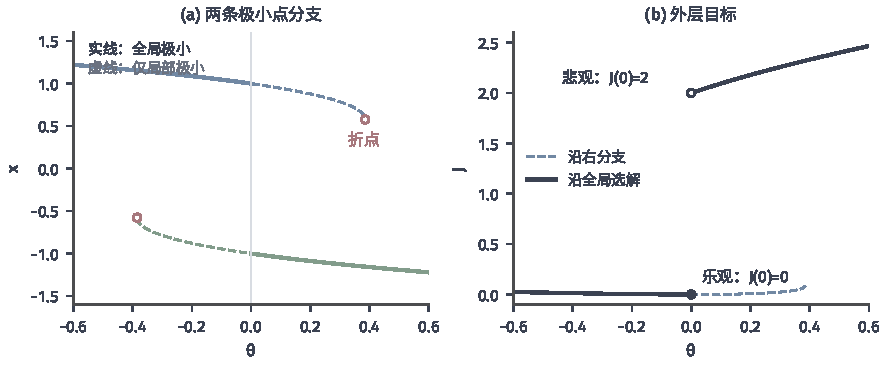
\includegraphics[width=150mm]{figures/03-optimization-evolution-and-signals/01-optimization/matplotlib/c7-branch-switch/figure.pdf}
  \caption{倾斜双势阱~\eqref{eq:opt-mmb-tilted-well}的内层分支与外层目标。(a)驻点方程$x^3-x+\theta=0$的两条局部极小点分支（右分支蓝、左分支绿）；实线段是全局极小点，虚线段只是局部极小点；空心圆是折点$\theta=\pm2/(3\sqrt3)$，此处Hessian$3x^2-1$为零。(b)外层值$\frac12(x-1)^2$：黑色实线沿全局选解，在$\theta=0$处跳变；蓝色虚线沿右分支，光滑地经过$\theta=0$。$\theta=0$处乐观规则取实心点$0$，悲观规则取空心点$2$。}
  \label{fig:opt-mmb-branch-switch}
\end{figure*}

因此，改变外层参数时，需要随时核验内层选解是否仍在同一可微分支，并且这条分支是否仍符合规定的选解规则。可行的做法包括：监测内层Hessian的最小特征值，接近零时警惕折点；在若干个$\bm\theta$处从不同初值重新求解内层，比较各局部解的内层值；分支切换时，不再使用跨越切换点的同一个隐式公式。报告结果时应同时给出所用的选解规则与分支、外层值，以及由引理~\ref{lem:opt-mmb-hypergradient-error}估计的超梯度误差。提高内层与伴随求解的精度，只能减小同一个目标上的数值误差；若把局部分支误当作全局选解，这是目标定义上的错误，再精确的计算也不能消除。
